\documentclass[11pt,]{article}
\usepackage[left=1in,top=1in,right=1in,bottom=1in]{geometry}
\newcommand*{\authorfont}{\fontfamily{phv}\selectfont}
\usepackage[]{mathpazo}


  \usepackage[T1]{fontenc}
  \usepackage[utf8]{inputenc}



\usepackage{abstract}
\renewcommand{\abstractname}{}    % clear the title
\renewcommand{\absnamepos}{empty} % originally center

\renewenvironment{abstract}
 {{%
    \setlength{\leftmargin}{0mm}
    \setlength{\rightmargin}{\leftmargin}%
  }%
  \relax}
 {\endlist}

\makeatletter
\def\@maketitle{%
  \newpage
%  \null
%  \vskip 2em%
%  \begin{center}%
  \let \footnote \thanks
    {\fontsize{18}{20}\selectfont\raggedright  \setlength{\parindent}{0pt} \@title \par}%
}
%\fi
\makeatother




\setcounter{secnumdepth}{3}


\usepackage{graphicx,grffile}
\makeatletter
\def\maxwidth{\ifdim\Gin@nat@width>\linewidth\linewidth\else\Gin@nat@width\fi}
\def\maxheight{\ifdim\Gin@nat@height>\textheight\textheight\else\Gin@nat@height\fi}
\makeatother
% Scale images if necessary, so that they will not overflow the page
% margins by default, and it is still possible to overwrite the defaults
% using explicit options in \includegraphics[width, height, ...]{}
\setkeys{Gin}{width=\maxwidth,height=\maxheight,keepaspectratio}

\title{Distribución espacial de los géneros y especies de la familia
\emph{Malvaceae} en una parcela de 50 ,ha. Caso: Isla Barro Colorado,
Panamá.  }



\author{\Large Ana Hilda Valera Arias\vspace{0.05in} \newline\normalsize\emph{Estudiante, Universidad Autónoma de Santo Domingo (UASD)}  }


\date{}

\usepackage{titlesec}

\titleformat*{\section}{\normalsize\bfseries}
\titleformat*{\subsection}{\normalsize\itshape}
\titleformat*{\subsubsection}{\normalsize\itshape}
\titleformat*{\paragraph}{\normalsize\itshape}
\titleformat*{\subparagraph}{\normalsize\itshape}

\titlespacing{\section}
{0pt}{36pt}{0pt}
\titlespacing{\subsection}
{0pt}{36pt}{0pt}
\titlespacing{\subsubsection}
{0pt}{36pt}{0pt}





\newtheorem{hypothesis}{Hypothesis}
\usepackage{setspace}

\makeatletter
\@ifpackageloaded{hyperref}{}{%
\ifxetex
  \PassOptionsToPackage{hyphens}{url}\usepackage[setpagesize=false, % page size defined by xetex
              unicode=false, % unicode breaks when used with xetex
              xetex]{hyperref}
\else
  \PassOptionsToPackage{hyphens}{url}\usepackage[unicode=true]{hyperref}
\fi
}

\@ifpackageloaded{color}{
    \PassOptionsToPackage{usenames,dvipsnames}{color}
}{%
    \usepackage[usenames,dvipsnames]{color}
}
\makeatother
\hypersetup{breaklinks=true,
            bookmarks=true,
            pdfauthor={Ana Hilda Valera Arias (Estudiante, Universidad Autónoma de Santo Domingo (UASD))},
             pdfkeywords = {Género, Planta},  
            pdftitle={Distribución espacial de los géneros y especies de la familia
\emph{Malvaceae} en una parcela de 50 ,ha. Caso: Isla Barro Colorado,
Panamá.},
            colorlinks=true,
            citecolor=blue,
            urlcolor=blue,
            linkcolor=magenta,
            pdfborder={0 0 0}}
\urlstyle{same}  % don't use monospace font for urls

% set default figure placement to htbp
\makeatletter
\def\fps@figure{htbp}
\makeatother

\usepackage{pdflscape} \newcommand{\blandscape}{\begin{landscape}}
\newcommand{\elandscape}{\end{landscape}}


% add tightlist ----------
\providecommand{\tightlist}{%
\setlength{\itemsep}{0pt}\setlength{\parskip}{0pt}}

\begin{document}
	
% \pagenumbering{arabic}% resets `page` counter to 1 
%
% \maketitle

{% \usefont{T1}{pnc}{m}{n}
\setlength{\parindent}{0pt}
\thispagestyle{plain}
{\fontsize{18}{20}\selectfont\raggedright 
\maketitle  % title \par  

}

{
   \vskip 13.5pt\relax \normalsize\fontsize{11}{12} 
\textbf{\authorfont Ana Hilda Valera Arias} \hskip 15pt \emph{\small Estudiante, Universidad Autónoma de Santo Domingo (UASD)}   

}

}








\begin{abstract}

    \hbox{\vrule height .2pt width 39.14pc}

    \vskip 8.5pt % \small 

\noindent Resumen del manuscrito


\vskip 8.5pt \noindent \emph{Keywords}: Género, Planta \par

    \hbox{\vrule height .2pt width 39.14pc}



\end{abstract}


\vskip 6.5pt


\noindent  \section{Introducción}\label{introducciuxf3n}

La vegetación terrestre está constituida por un conjunto de plantas
pertenecientes a una familia en específico y esta a su vez se subdividen
en géneros y especies para identificarse dentro de su clase. Por
consiguiente no sería la excepción de la \emph{malvaceae}, poseen 243
genéros y más de 4,300 especies, sus flores son hermafroditas, pocas
veces unisexuales, solitarias o fasciculadas en las axilas de las hojas
o agrupadas en inflorescencia tal como la describen los siguientes
autores (Marín, Hilario, \& Andino, n.d.) y (Bayer, 2003).

Dentro de los géneros a encontrar en la familia \emph{malvaceae} están
el \emph{abutilon} constituido por arbustos, subarbustos y hierbas
bienales con pelo estrellados y tallos velloso, son carente del epicáliz
conjunto de apéndices que por lo regular tienen otros grupos de dicha
familia, así como de tener alrededor de 150 especie nativa en los
trópicos y subtrópicos de América, África, Asia y Australia,
(Lorenzo-Cáceres, 2007). También, está el \emph{Hibiscus} donde los
segmentos del epicáliz estan libres o unidos en la base, con estigmas
alargados, semillas reniformes y numerosas, (ORTIZ, 2010). Del mismo
modo, se encuentra la \emph{althaea}, \emph{lavatera} y la \emph{malva}
cada una contienen sus respectivas especies las cuales pueden
encontrarse en mayor o menor proporción en un espacio determinado la
cual dependerá de factores abioticos incidentes entre ellos, lo que
implicaría la necesidad de utilizar tecnicas y análisis numerológicos
para conocer su asocianción y distribción.

La implementación de análisis numéricos en las investigaciones
ecológicas permiten dar a conocer en terminos cuantificables la forma en
que se encuentran asociadas y el tipo de patrón que presenta algunas
especies, es por ello la importancia de la estratificación y
zonificación del objeto de estudio en cuestión. De acuerdo con
(González, 2006) esto permite conjugar en un mismo grupo información de
aquellos organismos que pueden ser cuantificable junto con otros que son
reproductivos y de manera general con toda la vegetación.

En tal sentido, este estudio por medio de la ecología numérica busca
conocer cómo estan asociados los diferentes géneros y especies de la
familia \emph{malvaceae} y si las variables ambientales existente en la
zona influyen en dicha asociación. También, analizar como estan
organizados los grupos y qué patrón presentan en caso de que existiese y
asimismo establecer los indicadores ambientales que interfieren. De
igual manera, examinar en qué volumen se encuentran representadas cada
una y distiguir los sitios con especies alpha y beta, además, de
construir modelos de distribución espacial para idenficarla. Por
consiguiente, esta investigación constribuirá al conocimiento de la
dinámica ecológica espacial que envuelven las plantas pertenecientes a
la familia \emph{malvaceae} en la isla de Barro Colorado que en lo
adelante será llamado BCI y con la misma gestionar estrategias para el
cuidado y conservación de ésta.

\ldots

\section{Metodología}\label{metodologuxeda}

\subsection{Área de estudio}\label{uxe1rea-de-estudio}

La BCI se encuentra ubicada en el canal de Pánama en las proximidades
del lago Gatún, de acuerdo con (Pérez et al., 2005) esta se formó cuando
se construyó dicho canal embalsando las aguas del río Chagres, se
localiza entre las coordenadas geográficas (latitud 9\(^\circ\)~9'N,
longitud 79\(^\circ\)~ 50') y cubre una extensión de tierra de 1,500
hectáreas (ver figura \ref{mapa}). El clima es de bosque tropical, la
temperatura promedio es de 27 grados centígrados, con temporadas
lluviosas durante los meses mayo-diciembre y secas desde mediados de
diciembre hasta abril, las tormentas convectivas son prevenidas por los
vientos alisios dictando así las estaciones del año, (Sugasti, Eng, \&
Pinzón, 2018). Esta isla por sus caracteristicas fisicas sirve de
hábitat para muchos animales e insectos y por consiguiente para una
variedad de especie vegetal, convirtiendola en un espacio de
investigación de mucha importancia.

Es por ello, la escogencia como lugar de estudio la parcela permanente
de 50 hectárea de BCI donde se identificó como estan asociadas y
distribuidas la familia \emph{malvaceae} a través del censo realizado
por (Hubbell, Condit, \& Foster, 2021) durante varios años (1981-1983 y
2010-2015, entre otros) donde se identificaron, marcaron y
cartografiaron todos los tallos leñosos independientes de al menos 10 mm
de diámetro a la altura.

\begin{figure}
\centering
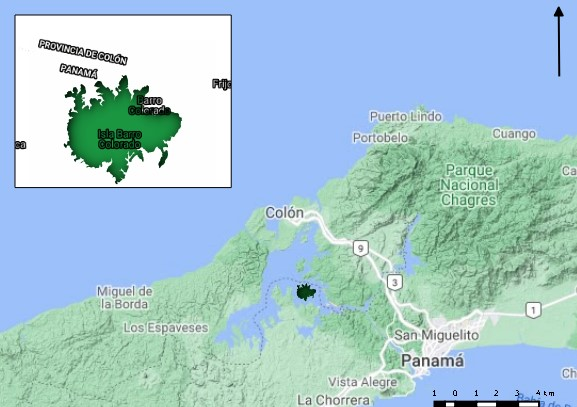
\includegraphics{mapa_barro_colorado.jpeg}
\caption{Ubicación de la isla Barro Colorado\label{mapa}}
\end{figure}

\subsubsection{Materiales y Técnicas de
investigación}\label{materiales-y-tuxe9cnicas-de-investigaciuxf3n}

Para la realización de este estudio se utilizó el software de (R Core
Team, 2019) donde se cargaron varios paquetes de ecología numérica como
el \emph{tidyverse} que ayudó a formar matriz de comunidad que permitió
identificar las diferentes especies que abundan, en qué cantidad y orden
de acuerdo a su pH. También, el \emph{Simple Features} (sf) para crear
área de hábitat por cuadros y obtener la densidad de cada especie por
metro cuadrado y así conocer la abundancia y riqueza global. De igual
manera, el \emph{Vegan} para caracterizar y analizar el orden y
disimilaridades entre cada especie y \emph{ez} para examinar las
unidades o variables repetitivas. Asimismo, el \emph{graphics},
\emph{psych} y \emph{mapvie} para la representación gráfica de cada
datos y (Kindt \& Coe, 2005) para señalar las especies alpha y beta,
cada \emph{script} utilizados fueron suministrado a partir del
repositorio de (Batlle, 2020) como fuente y el programa de información
geográfica Qgis (QGIS Development Team, 2009) para actualizar el mapa de
localización de la BCI.

\ldots

\section{Resultados}\label{resultados}

Por medio de los datos obtenidos a través del análisis de agrupamiento
se observó que existen 16 especies de la familia \emph{malvaceae} con
una distancia muy corta dentro de la 50,ha, dividido el espacio en dos
agrupos dentro de los cuales el uno tiene 42 sitio y el dos 8, siendo la
\emph{Quararibea asterolepis} la que más se asocia en el primero con
2,171 y la \emph{Sterculia apetala} en el segundo con 53 para un índice
de 0.015 respectivamente. En cuanto, al nivel de representación y
composición por cada 1,ha ha sido muy elevado en algunos puntos, como
muestra la matriz de \emph{Hellinger} en los cuadros 33 hasta el 49 de
los cluters donde la diferencia fueron extramadamente corta y la
similaridad numerosa, en tanto que, en el 8, 23, 30 y 35 fueron poco
similares y con un intervalo largo (ver figura \ref{representacion}). De
igual manera, en la diversidad de especie existó un alto rango de
correlación entre las riqueza y abundancia teniendo como resultado una
equidad en su distribución, como es el caso del índice de \emph{Hill}
aunque las riquezas aumentan o disminuyen la ratio no son afectadas.
También, se identificó que el sitio 30 es el de más riqueza en especie
alpha con 13 y el más pobre el 45 con 5 con una abundancia de 110 y 123
cosecutivamente, asimismo, los lugares que más varían son el 13 y 46,
estando las especies \emph{Apeiba membranacea}, \emph{Apeiba tibourbou},
\emph{Hampea appendiculata}, \emph{Herrania purpurea} entre otras como
beta con un valor de 0.07936325, 0.06962371, 0.13708297, 0.10517566
sucesivamente (ver figura \ref{diversidad} \& \ref{ambiente}). Además,
de existir insidencia de varios factores ambientales al aplicarse la
prueba \emph{Moran's} la cual mostró una correlación entre las especies
de manera positiva en la unidad geomorfológica del espolón, la vaguada y
la vertiente y de manera negativa en el piedemonte, el valle y la sima,
igualmente, con los componentes químicos como el \emph{calsio} (Ca),
\emph{cobre} (Cu), \emph{hierro} (Fe), \emph{zinc} (Zn), además, del
\emph{pH} siendo éste el más representativo desde el espacio 1 hasta el
7.

\begin{figure}
\centering
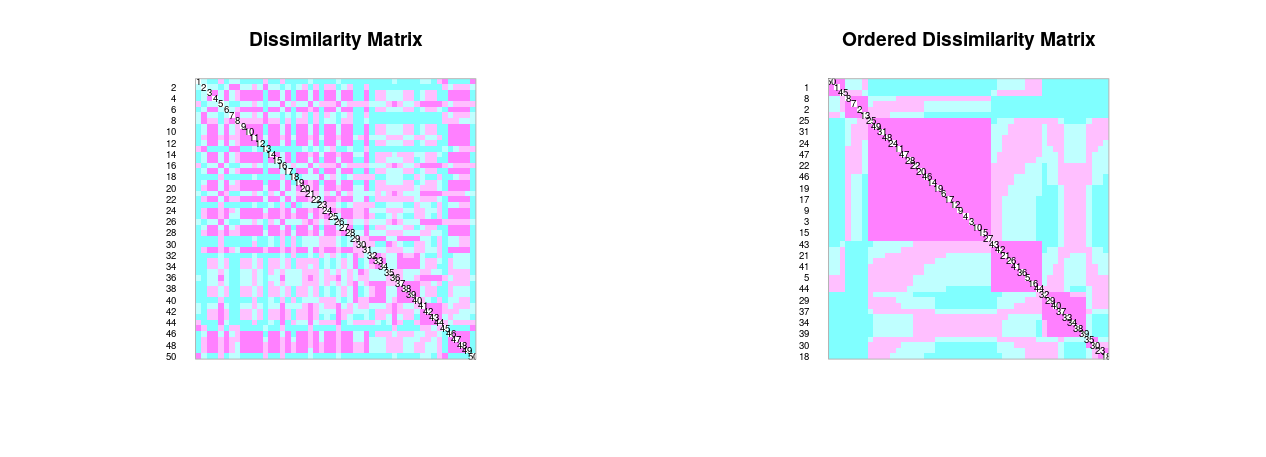
\includegraphics[width=1.00000\textwidth]{disimilaridad_Hellinger.png}
\caption{Composición de especies \emph{malvaceae} en cada sitio de la
BCI por distancia de cuerdas método Hellinger\label{representacion}}
\end{figure}

\begin{figure}
\centering
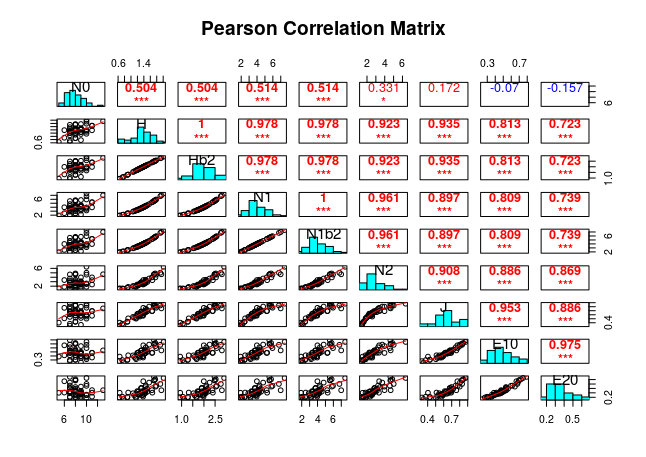
\includegraphics[width=1.20000\textwidth]{Matriz_correlacion_Pearson.png}
\caption{Correlación de las diferentes especies\label{diversidad}}
\end{figure}

\begin{figure}
\centering
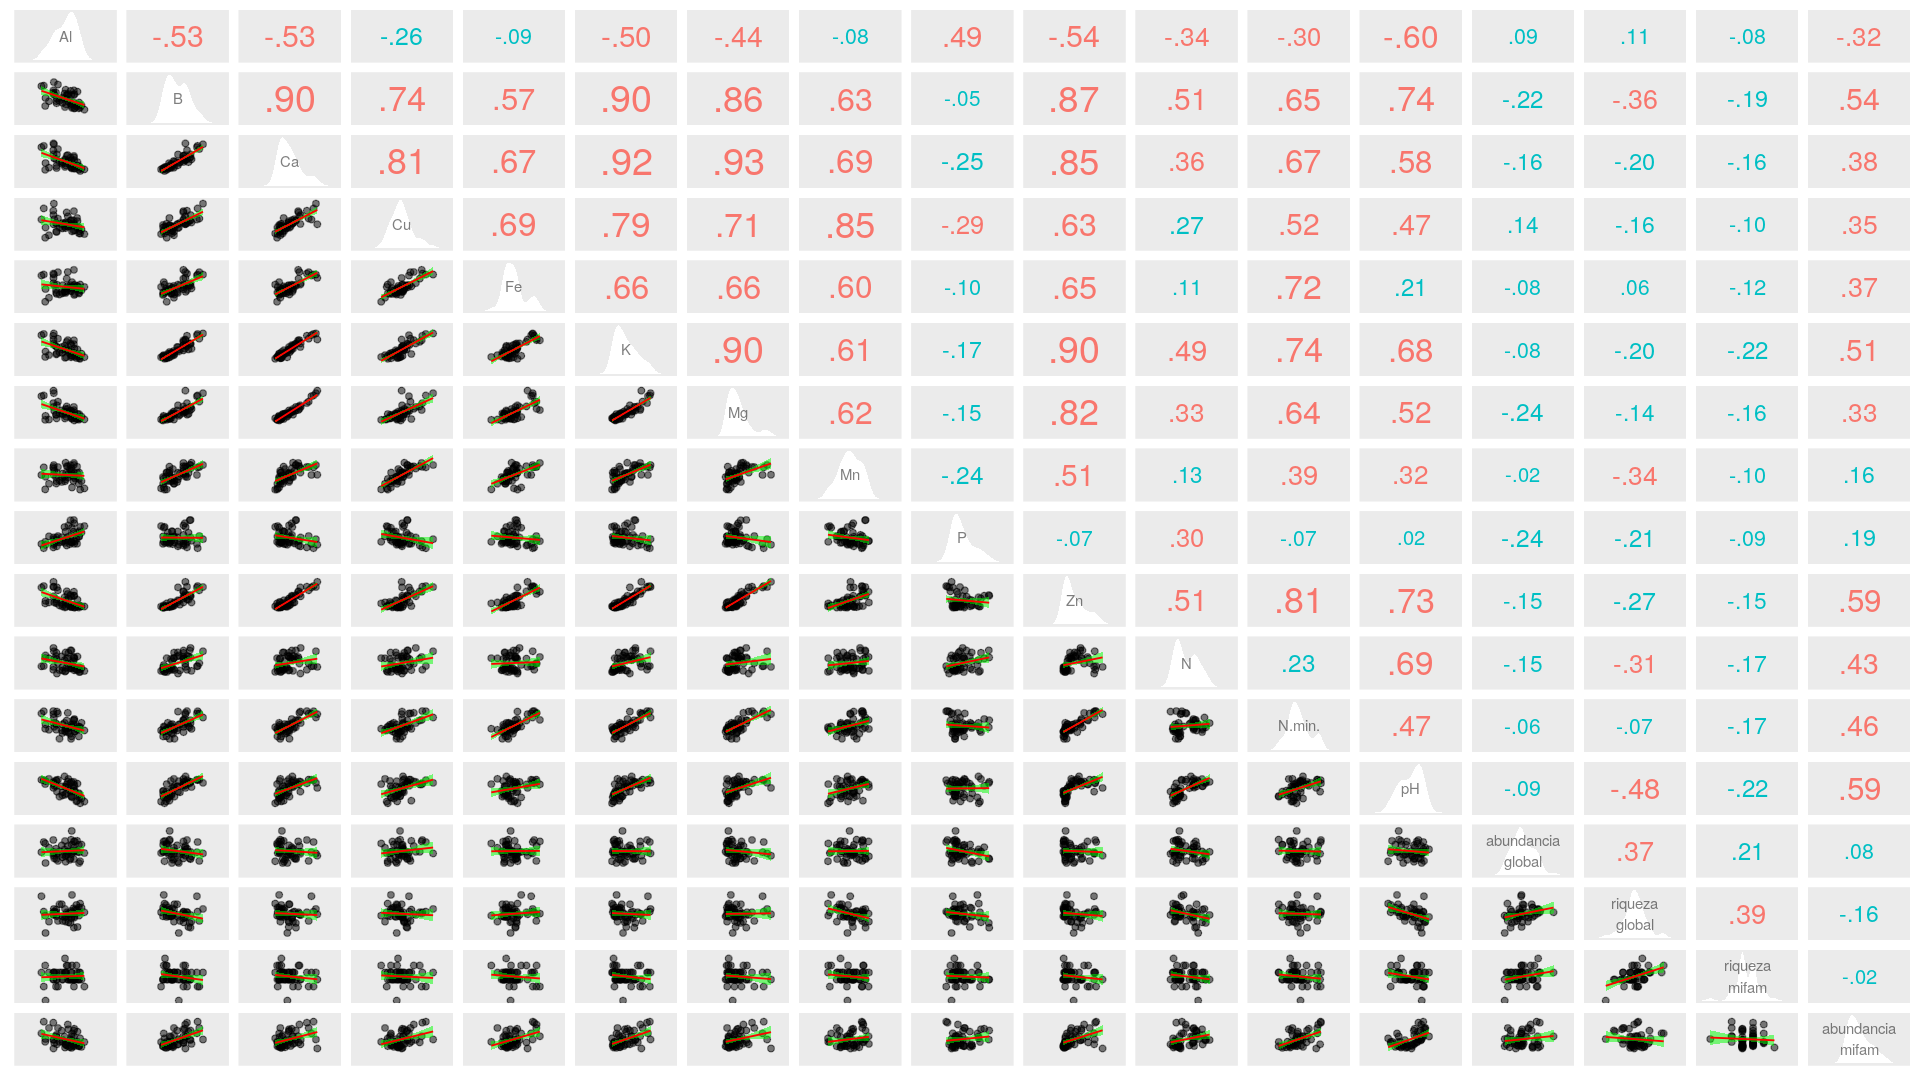
\includegraphics[width=1.10000\textwidth]{matriz_correlacion_suelo_abun_riq_spearman.png}
\caption{Correlación de las diferentes especies\label{ambiente}}
\end{figure}

\begin{figure}
\centering
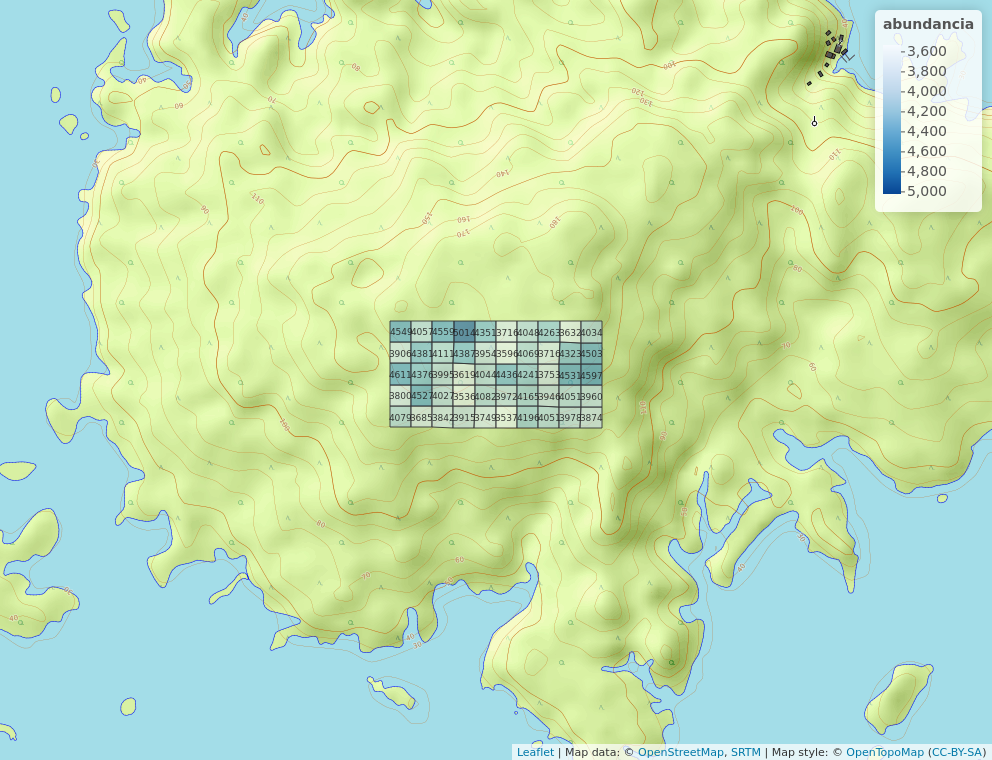
\includegraphics[width=1.10000\textwidth]{mapa_cuadros_abun_global.png}
\caption{Número de individuo por especie\label{riquezas}}
\end{figure}

\ldots

\section{Discusión}\label{discusiuxf3n}

La forma en que se encuentran distribuidos los géneros y especies de la
familia \emph{malvaceae} en la parcela de 50,h de la BCI se debe a
factores ambientales que influyen positivamente en su ordenación, auque
el exceso de ciertos elementos químicos pueden afectar la distribución y
crecimiento de ciertas plantas (Clark, 2002), como fue el caso de el
\emph{manganeso} (Mn), \emph{cobre} (Cu) y el \emph{aluminio} (Al) que
en su presencia la correlación con el espacio fue menor a diferencia del
\emph{zinc} (Zn), el \emph{boro} (B) y el \emph{potasio} (K) donde fue
mayor, a lo que se puede asumir que la abundancia o no de dichas
especies estuvieron influenciadas por el tipo de sustancia que más
existió en cada sitio. De igual manera, su organización espacial se vió
intervenida por la forma del relieve en algunas zonas, siendo la
Vaguada, el espolón y la vertiente los puntos que obtuvieron la mayor
riqueza en comparación con el piedemonte, el valle y la sima con menor,
posiblemente esto se deba al tipo de material presente en el terreno, ya
que, según (Flores, Suvires, \& Dalmasso, 2015) los suelos formados de
diferente roca madre o regolita, tienden a tener diferentes propiedades
tanto físicas como químicas, las cuales pueden ser beneficiosas para el
tipo de colocación actual. En cambio, la ausencia o baja proporción en
la que aparecen estas plantas en otras partes, sea por causa de su
formación, por ejemplo los espacios antes mencionados de menor
concentración por lo general son de origen detrítico-sedimentario,
transportados por corrientes fluviales efímeras con alta carga
sedimentaria y algunos aportes de arena eólica, (Flores et al., 2015),
lo que dificultaría la propagación de estas con el patrón observado.

\section{Agradecimientos}\label{agradecimientos}

\section{Información de soporte}\label{informaciuxf3n-de-soporte}

\ldots

\section{\texorpdfstring{\emph{Script}
reproducible}{Script reproducible}}\label{script-reproducible}

\ldots

\section*{Referencias}\label{referencias}
\addcontentsline{toc}{section}{Referencias}

\hypertarget{refs}{}
\hypertarget{ref-jose_ramon_martinez_batlle_2020_4402362}{}
Batlle, J. R. M. (2020).
Biogeografia-master/scripts-de-analisis-BCI;coding sessions (Version
v0.0.9000). \url{https://doi.org/10.5281/zenodo.4402362}

\hypertarget{ref-bayer2003malvaceae}{}
Bayer, K., Clemens y Kubitzki. (2003). Malvaceae. In Springer (Ed.),
\emph{Plantas con flores ~textperiodcentered dicotiledóneas}.

\hypertarget{ref-clark2002factores}{}
Clark, D. B. (2002). Los factores edáficos y la distribución de las
plantas. \emph{Ecología Y Conservación de Bosques Neotropicales. LUR,
Cartago, Costa Rica}, 193--221.

\hypertarget{ref-flores2015distribucion}{}
Flores, D. G., Suvires, G., \& Dalmasso, A. (2015). Distribución de la
vegetación nativa en ambientes geomorfológicos cuaternarios del monte
Árido central de argentina. \emph{Revista Mexicana de Biodiversidad},
\emph{86}(1), 72--79.

\hypertarget{ref-gonzalez2006ecologia}{}
González, A. R. (2006). \emph{Ecología: Métodos de muestreo y análisis
de poblaciones y comunidades}. Pontificia Universidad Javeriana.

\hypertarget{ref-webcenso}{}
Hubbell, S., Condit, R., \& Foster, R. (2021). \emph{Parcela del censo
forestal en la isla de barro colorado}.

\hypertarget{ref-biodiversidad}{}
Kindt, R., \& Coe, R. (2005). \emph{Tree diversity analysis. a manual
and software for common statistical methods for ecological and
biodiversity studies}. Retrieved from
\url{http://www.worldagroforestry.org/output/tree-diversity-analysis}

\hypertarget{ref-de2007especies}{}
Lorenzo-Cáceres, J. M. S. de. (2007). Las especies del género abutilon
mill.(Malvaceae) cultivadas en españa. \emph{PARJAP: Boletín de La
Asociación Española de Parques Y Jardines}, (45), 45--49.

\hypertarget{ref-marinanalisis}{}
Marín, J. Z., Hilario, R. F., \& Andino, O. O. (n.d.). \emph{Análisis
filogenético de la familia malvaceae}.

\hypertarget{ref-ortizclaves}{}
ORTIZ, D. G. (2010). \emph{Claves para los taxones y cultones del género
hibiscus l.(Malvaceae) cultivados y comercializados en la comunidad
valenciana (e españa)}.

\hypertarget{ref-perez2005metodologia}{}
Pérez, R., Aguilar, S., Condit, R., Foster, R., Hubbell, S., \& Lao, S.
(2005). Metodologia empleada en los censos de la parcela de 50 hectareas
de la isla de barro colorado, panamá. \emph{Centro de Ciencias
Forestales Del Tropico (CTFS) Y Instituto Smithsonian de Investigaciones
Tropicales (STRI)}, 1--24.

\hypertarget{ref-QGIS_software}{}
QGIS Development Team. (2009). \emph{QGIS geographic information
system}. Retrieved from \url{http://qgis.osgeo.org}

\hypertarget{ref-R}{}
R Core Team. (2019). \emph{R: A language and environment for statistical
computing}. Retrieved from \url{https://www.R-project.org/}

\hypertarget{ref-sugastimedicion}{}
Sugasti, L., Eng, B., \& Pinzón, R. (2018). \emph{Medición continúa de
flujo de co2 ensuelo en una parcela de bosque tropical en isla barro
colorado, canal de panamá.}




\newpage
\singlespacing 
\end{document}
